% PQC-LINK progress report 2: reliability, verification and preparation for Phase 2.
%
% Continues progress_report.tex (Report 1). Build (any LaTeX with TikZ and pgfplots):
%   latexmk -pdf progress_report_2.tex
% Regenerate the data files from the raw files first:
%   python3 -I prepare_data2.py ../../results CAPTURE_DIR data2 ../../build
% where CAPTURE_DIR was written by scripts/capture_demo.sh. Every number in the results
% sections comes from data2/numbers2.tex and the generated tables; do not type measurements here.
\documentclass[11pt,a4paper]{article}

\usepackage[margin=2.2cm]{geometry}
\usepackage[T1]{fontenc}
\usepackage{lmodern}
\usepackage{microtype}
\usepackage{xcolor}
\usepackage{booktabs}
\usepackage{tabularx}
\usepackage{array}
\usepackage{caption}
\usepackage{placeins}
\renewcommand{\topfraction}{0.9}\renewcommand{\floatpagefraction}{0.8}
\usepackage{tikz}
\usetikzlibrary{arrows.meta,positioning,fit,backgrounds,calc,decorations.pathreplacing}
\usepackage{pgfplots}
\usepgfplotslibrary{statistics}
\pgfplotsset{compat=1.17}
\usepackage[colorlinks=true,linkcolor=blue!50!black,urlcolor=blue!50!black]{hyperref}

% Generated by prepare_data2.py from the raw files. Do not edit.
\newcommand{\NHsA}{300}
\newcommand{\CliLatMedA}{0.943}
\newcommand{\CliLatPnfA}{1.715}
\newcommand{\CliCpuMedA}{0.580}
\newcommand{\CliCpuPnfA}{1.149}
\newcommand{\CliHeapMedA}{19.1}
\newcommand{\CliHeapPnfA}{19.2}
\newcommand{\SrvCpuMedA}{0.361}
\newcommand{\SrvCpuPnfA}{0.682}
\newcommand{\SrvHeapMedA}{15.2}
\newcommand{\SrvHeapPnfA}{15.2}
\newcommand{\SrvRxA}{273}
\newcommand{\SrvTxA}{755}
\newcommand{\CliTxA}{273}
\newcommand{\CliRxA}{755}
\newcommand{\SrvRssA}{8496}
\newcommand{\NHsB}{300}
\newcommand{\CliLatMedB}{1.124}
\newcommand{\CliLatPnfB}{1.919}
\newcommand{\CliCpuMedB}{0.716}
\newcommand{\CliCpuPnfB}{1.304}
\newcommand{\CliHeapMedB}{26.8}
\newcommand{\CliHeapPnfB}{27.0}
\newcommand{\SrvCpuMedB}{0.425}
\newcommand{\SrvCpuPnfB}{0.782}
\newcommand{\SrvHeapMedB}{21.1}
\newcommand{\SrvHeapPnfB}{21.3}
\newcommand{\SrvRxB}{1449}
\newcommand{\SrvTxB}{1843}
\newcommand{\CliTxB}{1449}
\newcommand{\CliRxB}{1843}
\newcommand{\SrvRssB}{8488}
\newcommand{\BytesAgree}{yes}
\newcommand{\SrvCpuRatio}{1.18}
\newcommand{\CliCpuRatio}{1.23}
\newcommand{\NTenSessions}{3}
\newcommand{\TenDate}{2026-10-20}
\newcommand{\TenCpu}{Intel(R) Core(TM) Ultra 9 285H}
\newcommand{\EightRuns}{18}
\newcommand{\EightPerCell}{3}
\newcommand{\EightDelivered}{18}
\newcommand{\EightRejected}{0}
\newcommand{\EightRecords}{200}
\newcommand{\EightRate}{20}
\newcommand{\EightMtu}{1500}
\newcommand{\EightDate}{2026-10-20}
\newcommand{\EightMaxLoss}{30}
\newcommand{\WireAOver}{1456}
\newcommand{\WireAPkts}{22}
\newcommand{\WireARetx}{0}
\newcommand{\WireAAgree}{yes}
\newcommand{\WireAGroups}{001d}
\newcommand{\WireASuite}{1301}
\newcommand{\WireAChosen}{001d}
\newcommand{\WireBOver}{1456}
\newcommand{\WireBPkts}{22}
\newcommand{\WireBRetx}{0}
\newcommand{\WireBAgree}{yes}
\newcommand{\WireBGroups}{11ec}
\newcommand{\WireBSuite}{1301}
\newcommand{\WireBChosen}{11ec}
\newcommand{\TamperLost}{1}
\newcommand{\TamperAcked}{5}
\newcommand{\TamperTampered}{1}
\newcommand{\TamperServerErr}{1}
\newcommand{\TamperDup}{0}
\newcommand{\NTests}{22}


% Palette: A = classical (blue), B = hybrid (orange); state colours for the diagrams.
\definecolor{colorA}{RGB}{31,119,180}
\definecolor{colorB}{RGB}{214,95,0}
\definecolor{okgreen}{RGB}{34,120,60}
\definecolor{badred}{RGB}{176,32,32}

\tikzset{
  box/.style={draw, rounded corners=2pt, minimum height=8mm, align=center,
              font=\small, fill=white, line width=0.6pt, inner sep=3pt},
  done/.style={box, draw=okgreen, fill=okgreen!8},
  newd/.style={box, draw=okgreen, fill=okgreen!22, line width=0.9pt},
  todo/.style={box, draw=black!55, dashed, fill=black!4},
  next/.style={box, draw=colorB!85!black, densely dotted, fill=colorB!8},
  bad/.style={box, draw=badred, fill=badred!7},
  arr/.style={-{Stealth[length=2.2mm]}, line width=0.6pt},
  darr/.style={{Stealth[length=2.2mm]}-{Stealth[length=2.2mm]}, line width=0.6pt},
  badarr/.style={-{Stealth[length=2.2mm]}, line width=0.6pt, badred, dashed},
  lbl/.style={font=\scriptsize, fill=white, inner sep=1.2pt},
  note/.style={font=\scriptsize, align=left, text width=3.9cm},
  life/.style={line width=0.5pt, black!55},
  by/.style={draw, minimum height=7mm, inner sep=0pt, font=\tiny, align=center, anchor=west},
}

\captionsetup{font=small,labelfont=bf}
\setlength{\parindent}{0pt}
\setlength{\parskip}{0.55em}

\newcommand{\prog}[1]{\texttt{#1}}
\newcommand{\msg}[1]{\textsc{#1}}

\title{\textbf{PQC-LINK: Progress Report 2}\\[2pt]
       \large Reliable delivery, verification on the wire, and preparation for Phase~2}
\author{RSCL senior design team}
\date{\today}

\begin{document}
\maketitle

\begin{abstract}
\noindent Report~1 described the secure link itself: a TLS~1.3 client and server that compare
classical key exchange (configuration~A, \prog{X25519}) with hybrid post-quantum key exchange
(configuration~B, \prog{X25519MLKEM768}), and a first handshake benchmark. Since then the team
added what the link needs to be useful: a durable store on the receiving side, a persistent queue
on the sending side, tests for outages, restarts and packet loss, and the server's half of the
handshake cost. We also checked what actually crosses the wire with a real packet capture and
damaged encrypted records on purpose to see that they are refused. Finally we started the
Phase~2 software that needs no hardware: the UART frame format and the code that turns sensor
frames into records. Everything here was measured or tested on one development computer over
loopback. None of it is gate evidence, and the numbers are \emph{preliminary}.
\end{abstract}

\section{Since Report 1}

Report~1 ended with a working link, a failure-case test suite and a benchmark harness; the
durable store, the queue and the loss tests were listed as ``next'' or ``planned''.
Table~\ref{tab:since} shows what changed, and Figure~\ref{fig:map} shows the same on a map of the
system. The automated test suite grew from 10 tests to \NTests{}.

\begin{table}[!htbp]
\centering
\caption{Status against Report~1. ``Tested'' means automated tests pass on the development computer.}
\label{tab:since}
\small
\begin{tabularx}{\linewidth}{@{}lXl@{}}
\toprule
Area & What exists now & State \\
\midrule
Durable store, dedup & Append-only file, \prog{fsync} before the ACK, duplicate recognised by node and sequence & Tested \\
Persistent queue & Append-only file, sequence numbers owned by the queue, ACK entries, atomic compaction & Tested \\
Client resend & Window of 32, reconnect with backoff, resend from the oldest un-ACKed record & Tested \\
Outage, restart, overflow & T05, T06, T07 and the queue-full case run as real processes & Tested \\
Packet-loss runs (T08) & Runner with \prog{tc netem} at 0, 10, 30\,\%, no root needed & First look \\
Handshake cost (T10) & Client \emph{and} server CPU, memory and bytes & First look \\
On the wire & Real packet capture; damaged records refused over real TCP (T09) & Tested \\
UART frame, sample source & Frame format, parser, gap counting; the Pico side shares the code & Tested \\
Pico firmware, IMU, OLED, Wi-Fi & Phase 2, after the advisor reviews Phase 1 & Deferred \\
\bottomrule
\end{tabularx}
\end{table}

\begin{figure}[!tbp]
\centering
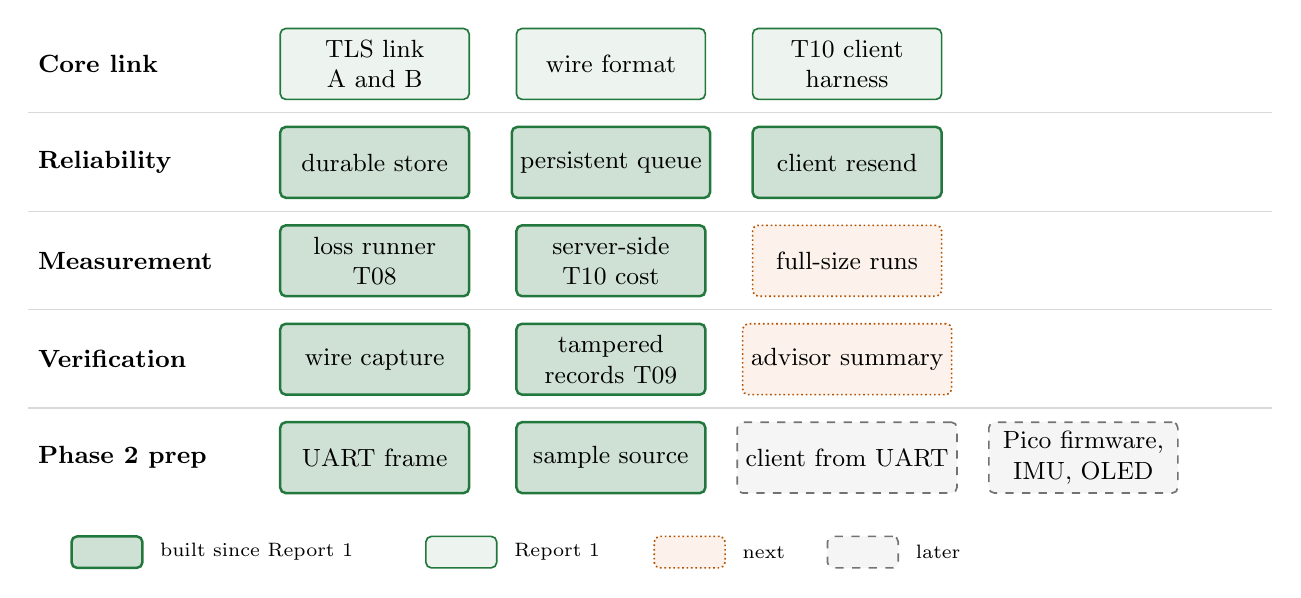
\begin{tikzpicture}[every node/.append style={font=\scriptsize}]
  \tikzset{cell/.style={minimum width=2.4cm, minimum height=9mm}}
  \foreach \y/\t in {0/Core link, -1.25/Reliability, -2.5/Measurement, -3.75/Verification, -5.0/Phase 2 prep}
    \node[font=\small\bfseries, anchor=west] at (0,\y) {\t};
  \foreach \y in {-0.62,-1.87,-3.12,-4.37}
    \draw[black!15, line width=0.4pt] (0,\y) -- (15.8,\y);
  % columns at x = 4.4, 7.2, 10.0, 12.8
  \node[done, cell] at (4.4,0) {TLS link\\A and B};
  \node[done, cell] at (7.4,0) {wire format};
  \node[done, cell] at (10.4,0) {T10 client\\harness};
  \node[newd, cell] at (4.4,-1.25) {durable store};
  \node[newd, cell] at (7.4,-1.25) {persistent queue};
  \node[newd, cell] at (10.4,-1.25) {client resend};
  \node[newd, cell] at (4.4,-2.5) {loss runner\\T08};
  \node[newd, cell] at (7.4,-2.5) {server-side\\T10 cost};
  \node[next, cell] at (10.4,-2.5) {full-size runs};
  \node[newd, cell] at (4.4,-3.75) {wire capture};
  \node[newd, cell] at (7.4,-3.75) {tampered\\records T09};
  \node[next, cell] at (10.4,-3.75) {advisor summary};
  \node[newd, cell] at (4.4,-5.0) {UART frame};
  \node[newd, cell] at (7.4,-5.0) {sample source};
  \node[todo, cell] at (10.4,-5.0) {client from UART};
  \node[todo, cell] at (13.4,-5.0) {Pico firmware,\\IMU, OLED};
  % legend
  \node[newd, minimum width=9mm, minimum height=4mm] at (1.0,-6.2) {};
  \node[anchor=west] at (1.55,-6.2) {built since Report 1};
  \node[done, minimum width=9mm, minimum height=4mm] at (5.5,-6.2) {};
  \node[anchor=west] at (6.05,-6.2) {Report 1};
  \node[next, minimum width=9mm, minimum height=4mm] at (8.4,-6.2) {};
  \node[anchor=west] at (8.95,-6.2) {next};
  \node[todo, minimum width=9mm, minimum height=4mm] at (10.6,-6.2) {};
  \node[anchor=west] at (11.15,-6.2) {later};
\end{tikzpicture}
\caption{Progress map. Dark green: built since Report~1.}
\label{fig:map}
\end{figure}

\section{Decisions since Report 1}

Table~\ref{tab:decisions} lists the design decisions made since Report~1. Those marked
\emph{proposed} are written in the protocol document with the value we suggest; they need the
advisor's confirmation.

\begin{table}[!htbp]
\centering
\caption{Decisions. ``Team'' = decided by the team; ``proposed'' = written down, awaiting the advisor.}
\label{tab:decisions}
\small
\begin{tabularx}{\linewidth}{@{}X>{\raggedright\arraybackslash}p{1.7cm}X@{}}
\toprule
Decision & Status & Why \\
\midrule
Durable files are append-only with a check value per entry; only a torn \emph{last} entry is
cut off, any other damage stops the program & Team &
A power cut can only tear the last write; anything else would lose acknowledged data \\
Not SQLite: a plain file with one \prog{fsync} per record & Team & No new dependency, every
durability step is short and tested \\
The queue owns the sequence numbers; a header floor stops a number being reused after compaction
& Team & A reused number would be treated as a duplicate and lose data \\
Queue holds 10{,}000 un-ACKed records; a full queue rejects, counts, and still uses up the number
& Proposed & Never drop a record already promised; the gap shows the loss \\
A handshake that times out is retried; an alert, a failed verification or a policy mismatch is
never retried & Team & Packet loss must not end a run, but a retry loop must not hide T03 or T04 \\
Pico~2 or Pico~W does sensor and display I/O only; Pico firmware is C with the Pico SDK
& Team, confirm & They cannot run TLS; all TLS stays on the Pi~4B \\
Code shared with the firmware may use only the standard integer types and the error codes
& Team & Both ends then compile the same file and cannot disagree about the format \\
\bottomrule
\end{tabularx}
\end{table}

\section{Reliable delivery}

\subsection{The path of one record}

The rule behind the design is: \emph{a side may forget a record only after the other side holds
it durably}. Figure~\ref{fig:journey} shows it. The sender writes a record to its queue file and
forces it to disk before sending; the receiver writes it to its store and forces it to disk
before acknowledging; the sender removes the record only after the acknowledgement arrives. If an
acknowledgement is lost, the sender sends the record again and the receiver recognises it by its
node and sequence number, acknowledges again, and changes nothing else. The count shown on the
display therefore cannot go up twice for one record.

\begin{figure}[!tbp]
\centering
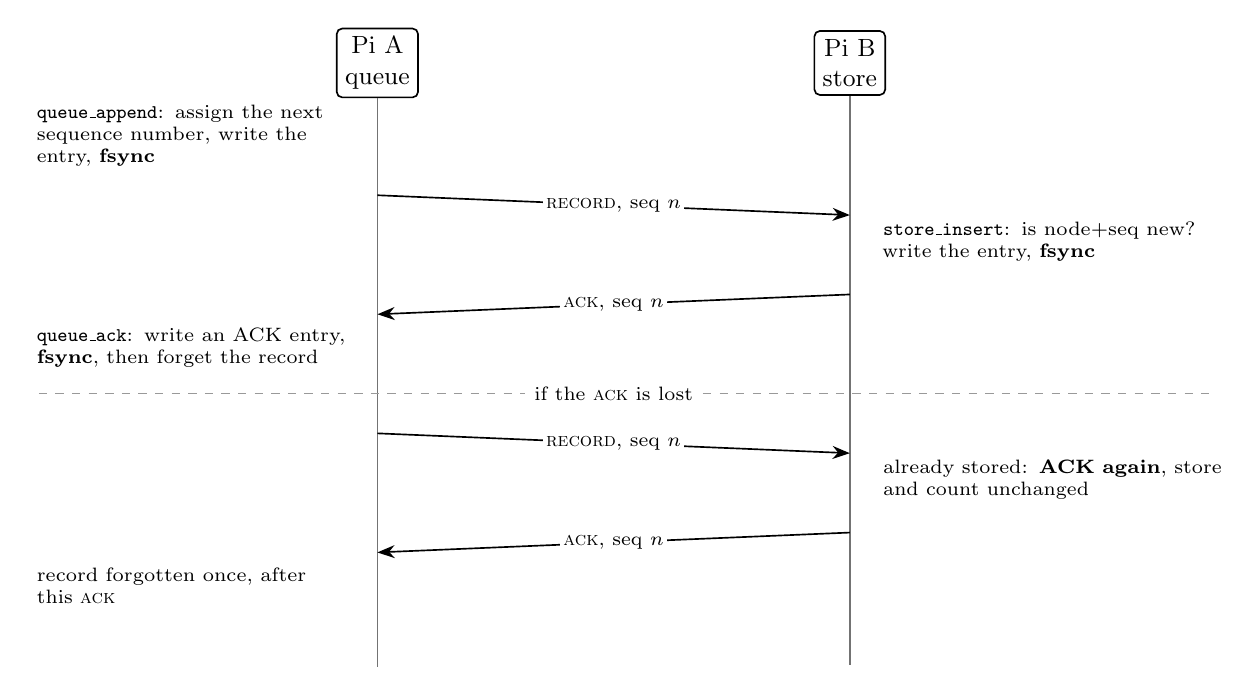
\begin{tikzpicture}[x=1cm,y=0.84cm]
  \node[box] (A) at (4.3,0) {Pi A\\queue};
  \node[box] (B) at (10.3,0) {Pi B\\store};
  \draw[life] (A.south) -- ++(0,-8.6);
  \draw[life] (B.south) -- ++(0,-8.6);
  % normal path
  \node[note, anchor=east] at (4.0,-1.1) {\prog{queue\_append}: assign the next sequence number, write the entry, \textbf{fsync}};
  \draw[arr] (4.3,-2.0) -- node[lbl] {\msg{record}, seq $n$} (10.3,-2.3);
  \node[note, anchor=west, text width=4.3cm] at (10.6,-2.7) {\prog{store\_insert}: is node+seq new? write the entry, \textbf{fsync}};
  \draw[arr] (10.3,-3.5) -- node[lbl] {\msg{ack}, seq $n$} (4.3,-3.8);
  \node[note, anchor=east] at (4.0,-4.3) {\prog{queue\_ack}: write an ACK entry, \textbf{fsync}, then forget the record};
  \draw[dashed, black!40] (0,-5.0) -- (14.9,-5.0);
  \node[font=\scriptsize, fill=white] at (7.3,-5.0) {if the \msg{ack} is lost};
  % lost-ack path
  \draw[arr] (4.3,-5.6) -- node[lbl] {\msg{record}, seq $n$} (10.3,-5.9);
  \node[note, anchor=west, text width=4.3cm] at (10.6,-6.3) {already stored: \textbf{ACK again}, store and count unchanged};
  \draw[arr] (10.3,-7.1) -- node[lbl] {\msg{ack}, seq $n$} (4.3,-7.4);
  \node[note, anchor=east] at (4.0,-7.9) {record forgotten once, after this \msg{ack}};
\end{tikzpicture}
\caption{One record, with the two points where data is forced to disk.}
\label{fig:journey}
\end{figure}

\subsection{On disk}

Both files are logs that are only added to. Figure~\ref{fig:files} shows their layout. An entry is
a message exactly as it travels on the network plus a four-byte check value (CRC-32). The queue
needs a second kind of entry, an ACK, and a small header holding a \emph{floor} for the next
sequence number: compaction (writing a new file with only the waiting records and renaming it over
the old one) drops the entries that mention old numbers, and without the floor a restart could
hand the same number out again.

\begin{figure}[!tbp]
\centering
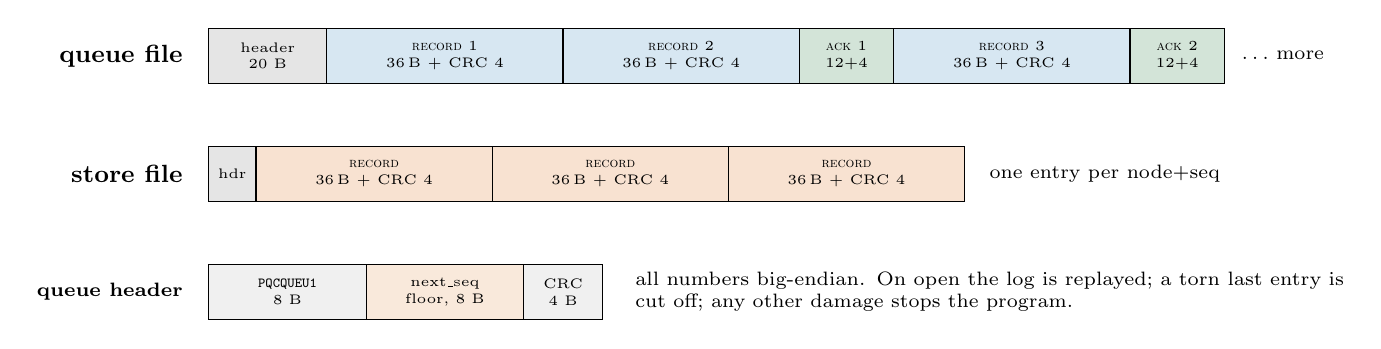
\begin{tikzpicture}[x=1cm,y=1cm]
  % one byte = 0.075 cm; positions below are in cm
  \node[font=\small\bfseries, anchor=east] at (-0.2,0) {queue file};
  \node[by, minimum width=1.5cm, fill=black!10] at (0,0) {header\\20 B};
  \node[by, minimum width=3.0cm, fill=colorA!18] at (1.5,0) {\msg{record} 1\\36\,B + CRC 4};
  \node[by, minimum width=3.0cm, fill=colorA!18] at (4.5,0) {\msg{record} 2\\36\,B + CRC 4};
  \node[by, minimum width=1.2cm, fill=okgreen!20] at (7.5,0) {\msg{ack} 1\\12+4};
  \node[by, minimum width=3.0cm, fill=colorA!18] at (8.7,0) {\msg{record} 3\\36\,B + CRC 4};
  \node[by, minimum width=1.2cm, fill=okgreen!20] at (11.7,0) {\msg{ack} 2\\12+4};
  \node[font=\scriptsize, anchor=west] at (13.0,0) {$\ldots$ more};
  \node[font=\small\bfseries, anchor=east] at (-0.2,-1.5) {store file};
  \node[by, minimum width=0.6cm, fill=black!10] at (0,-1.5) {hdr};
  \node[by, minimum width=3.0cm, fill=colorB!18] at (0.6,-1.5) {\msg{record}\\36\,B + CRC 4};
  \node[by, minimum width=3.0cm, fill=colorB!18] at (3.6,-1.5) {\msg{record}\\36\,B + CRC 4};
  \node[by, minimum width=3.0cm, fill=colorB!18] at (6.6,-1.5) {\msg{record}\\36\,B + CRC 4};
  \node[font=\scriptsize, anchor=west] at (9.8,-1.5) {one entry per node+seq};
  \node[font=\scriptsize\bfseries, anchor=east] at (-0.2,-3.0) {queue header};
  \node[by, minimum width=2.0cm, fill=black!6] at (0,-3.0) {\texttt{PQCQUEU1}\\8 B};
  \node[by, minimum width=2.0cm, fill=colorB!14] at (2.0,-3.0) {next\_seq\\floor, 8 B};
  \node[by, minimum width=1.0cm, fill=black!6] at (4.0,-3.0) {CRC\\4 B};
  \node[font=\scriptsize, anchor=west, text width=9cm] at (5.3,-3.0) {all numbers big-endian. On open the log is replayed; a torn last entry is cut off; any other damage stops the program.};
\end{tikzpicture}
\caption{Queue and store files. A record is waiting in the queue if no ACK entry follows it.}
\label{fig:files}
\end{figure}

\subsection{What a crash does}

Table~\ref{tab:crash} lists the failures the tests inject and what the code does. The queue was
also checked against a model: 3000 random appends, ACKs (in order, repeated and out of order) and
restarts compared with a plain array, and no sequence number is ever reused.

\begin{table}[!htbp]
\centering
\caption{Crash and damage cases, all covered by automated tests.}
\label{tab:crash}
\small
\begin{tabularx}{\linewidth}{@{}XX@{}}
\toprule
What happens & Result \\
\midrule
Power cut in the middle of writing the last entry & Entry cut off at start; it was never acknowledged, so nothing is lost \\
Server stores a record, ACK never arrives & Client resends; server acknowledges again; counted once (T05) \\
Client stopped (or killed with SIGKILL) with records waiting & On restart the waiting records are sent first; numbering carries on (T07) \\
Server down for the whole run & Queue grows, then drains after reconnect (T06) \\
Queue full & New records rejected and counted; the gap in sequence numbers shows the loss \\
Damage anywhere before the last entry, a repeated number, a file that is not a queue & Program refuses to start; the file is left untouched \\
Crash during compaction & Old file or new file, whole, never a mix \\
\bottomrule
\end{tabularx}
\end{table}

\FloatBarrier
\section{Packet loss (T08)}

\subsection{Method}

Loss is emulated with \prog{tc netem} on the loopback interface. Doing that normally needs root. The
runner (Figure~\ref{fig:lossrig}) instead starts the server and the client inside a fresh, unprivileged
user and network namespace, where the team has its own loopback and the right to change it. Runs
cannot disturb each other or the machine, and the namespace's TCP counters hold exactly one run. The
loopback is set to the Ethernet MTU of 1500 bytes, so a long message is split into packets as it would
be on Wi-Fi. Loss applies to every packet in both directions, so a request and its answer can each be
lost.

\begin{figure}[!tbp]
\centering
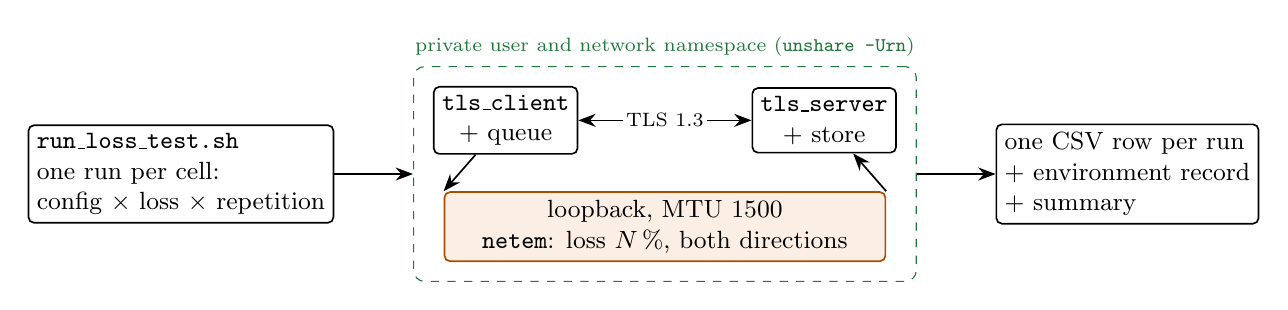
\begin{tikzpicture}[node distance=5mm and 8mm]
  \node[box] (cli) {\prog{tls\_client}\\+ queue};
  \node[box, right=22mm of cli] (srv) {\prog{tls\_server}\\+ store};
  \node[box, fill=colorB!10, draw=colorB!80!black, below=9mm of $(cli)!0.5!(srv)$, minimum width=5.6cm] (lo)
       {loopback, MTU 1500\\\prog{netem}: loss $N\,\%$, both directions};
  \draw[darr] (cli) -- node[lbl] {TLS 1.3} (srv);
  \draw[arr] (cli) -- (lo.north west);
  \draw[arr] (lo.north east) -- (srv);
  \begin{scope}[on background layer]
    \node[draw=okgreen, dashed, rounded corners=4pt, fit=(cli)(srv)(lo), inner sep=7pt,
          label={[font=\scriptsize, okgreen]above:private user and network namespace (\prog{unshare -Urn})}] (ns) {};
  \end{scope}
  \node[box, left=10mm of ns, align=left] (run) {\prog{run\_loss\_test.sh}\\one run per cell:\\config $\times$ loss $\times$ repetition};
  \node[box, right=10mm of ns, align=left] (csv) {one CSV row per run\\+ environment record\\+ summary};
  \draw[arr] (run) -- (ns);
  \draw[arr] (ns) -- (csv);
\end{tikzpicture}
\caption{The loss runner. A and B alternate within each loss level so drift hits both equally.}
\label{fig:lossrig}
\end{figure}

A run counts as \emph{delivered} only if nothing is still waiting in the queue, the number of
records the server stored equals the number the client accepted, and the client's count of ACKs
agrees. The server's count is read from the size of its store file, not from its log. Every run is
reported, delivered or not; a result with fewer than 10 runs per cell is marked insufficient.

\subsection{First look}

Table~\ref{tab:loss} and Figure~\ref{fig:drain} show one development-sized matrix: \EightPerCell{}
repetitions per cell, \EightRecords{} records per run at \EightRate{}\,Hz, \EightRuns{} runs in total,
measured on \EightDate{}. This is far below the 10 repetitions of 10 minutes that the specification asks
for, so \textbf{none of these numbers is a result}; they show that the runner works and what to expect.
Out of \EightRuns{} runs, \EightDelivered{} delivered every accepted record and \EightRejected{}
records were rejected by a full queue.

\begin{table}[!htbp]
\centering
\caption{T08, development-sized. Medians over the repetitions of each cell. Drain time is the time
from the last record made until nothing is waiting. Retransmissions are TCP segments, read from the
namespace's own counters: they show the emulated loss acted.}
\label{tab:loss}
\small
\begin{tabular}{@{}llrrrrrrr@{}}
\toprule
Config & Loss & Runs & Delivered & Lost sessions & TCP retrans. & Drain, ms & Drain p95, ms & Run, s \\
\midrule
% Generated by prepare_data2.py. Do not edit.
A & 0\,\% & 3 & 3 & 0 & 0 & 6 & 10 & 10.0 \\
B & 0\,\% & 3 & 3 & 0 & 0 & 6 & 8 & 10.0 \\
A & 10\,\% & 3 & 3 & 0 & 51 & 14 & 80 & 10.0 \\
B & 10\,\% & 3 & 3 & 0 & 43 & 16 & 21 & 10.0 \\
A & 30\,\% & 3 & 3 & 3 & 76 & 5\,114 & 53\,151 & 15.8 \\
B & 30\,\% & 3 & 3 & 1 & 70 & 3\,591 & 19\,371 & 14.2
\\
\bottomrule
\end{tabular}
\end{table}

\begin{figure}[!tbp]
\centering
\begin{tikzpicture}
  \begin{axis}[ybar, width=0.7\linewidth, height=5.6cm, bar width=14pt,
      xlabel={emulated loss, \%}, ylabel={median drain time, ms},
      xtick={0,10,30}, xmin=-8, xmax=38, ymode=log, ymin=1, log origin=infty,
      legend style={at={(0.03,0.97)}, anchor=north west, font=\scriptsize},
      axis lines=left, ymajorgrids, grid style={black!12}]
    \addplot[fill=colorA!35, draw=colorA!80!black] table[col sep=comma, x=loss, y=A] {data2/loss_drain.csv};
    \addplot[fill=colorB!35, draw=colorB!80!black] table[col sep=comma, x=loss, y=B] {data2/loss_drain.csv};
    \legend{A: X25519, B: X25519MLKEM768}
  \end{axis}
\end{tikzpicture}
\caption{Median time to empty the queue after the last record, by emulated loss. The vertical axis is logarithmic: at 0\,\% and 10\,\% the queue empties in milliseconds, at 30\,\% in seconds.}
\label{fig:drain}
\end{figure}

\section{The cost of a handshake, on both ends}

Report~1 measured only the client. The server now writes one row per accepted connection
(Figure~\ref{fig:twosides}): the CPU time of the server process over the handshake call itself
(waiting for the client is not counted), the heap the open connection holds, the handshake bytes, and
the process's peak memory. Rows are written after the timed span, never inside it. The summary drops
failed and warm-up rows and refuses to continue if the server's count differs from the client's.

\begin{figure}[!tbp]
\centering
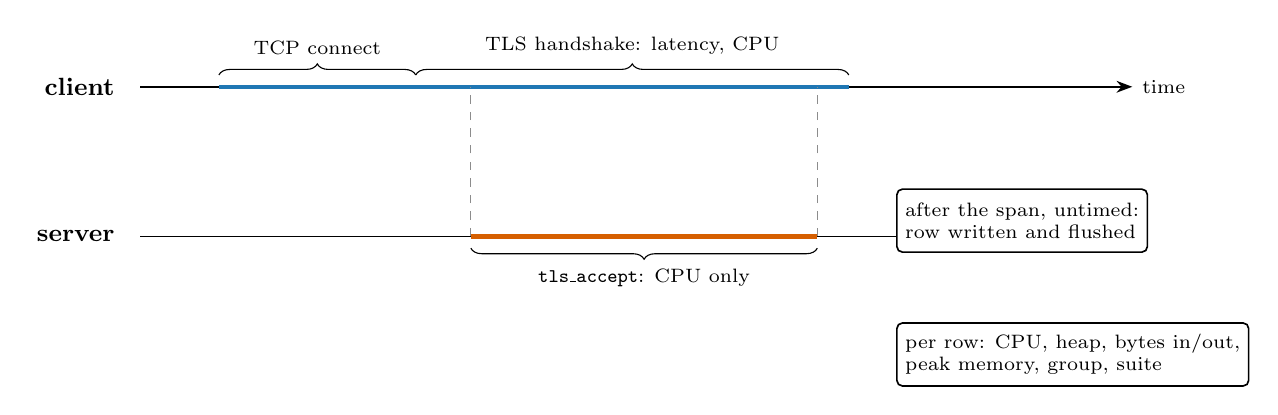
\begin{tikzpicture}[x=1cm,y=1cm]
  \node[font=\small\bfseries, anchor=east] at (-0.2,1.9) {client};
  \node[font=\small\bfseries, anchor=east] at (-0.2,0) {server};
  \draw[-{Stealth}, line width=0.6pt] (0,1.9) -- (12.6,1.9) node[right, font=\scriptsize] {time};
  \draw[-{Stealth}, line width=0.6pt] (0,0) -- (12.6,0);
  \draw[decorate, decoration={brace, amplitude=4pt}] (1,2.05) -- node[above=4pt, font=\scriptsize] {TCP connect} (3.5,2.05);
  \draw[decorate, decoration={brace, amplitude=4pt}] (3.5,2.05) -- node[above=4pt, font=\scriptsize] {TLS handshake: latency, CPU} (9,2.05);
  \draw[decorate, decoration={brace, amplitude=4pt, mirror}] (4.2,-0.15) -- node[below=4pt, font=\scriptsize] {\prog{tls\_accept}: CPU only} (8.6,-0.15);
  \draw[colorB, line width=1.6pt] (4.2,0) -- (8.6,0);
  \draw[colorA, line width=1.6pt] (1,1.9) -- (9,1.9);
  \draw[dashed, black!45] (4.2,0) -- (4.2,1.9);
  \draw[dashed, black!45] (8.6,0) -- (8.6,1.9);
  \node[box, align=left, font=\scriptsize, anchor=west] at (9.6,0.2) {after the span, untimed:\\row written and flushed};
  \node[box, align=left, font=\scriptsize, anchor=west] at (9.6,-1.5) {per row: CPU, heap, bytes in/out,\\peak memory, group, suite};
\end{tikzpicture}
\caption{What each side measures. Neither writes anything during its timed span.}
\label{fig:twosides}
\end{figure}

\subsection{Conditions}

\begin{itemize}\setlength\itemsep{0pt}
\item Platform: \TenCpu, WSL2; client and both servers on one machine over loopback, Release build.
\item \NTenSessions{} sessions, \NHsA{} measured handshakes per configuration in total; run date \TenDate.
\item Both sides counted the same bytes in every handshake (client sent = server received and the
      reverse): \BytesAgree.
\end{itemize}

\textbf{Preliminary:} one development computer, loopback, no loss.

\subsection{First look}

Table~\ref{tab:both} puts the two sides next to each other. In this run the hybrid handshake cost the
server about \SrvCpuRatio{} times the CPU time of the classical one, and the client about
\CliCpuRatio{} times. The open connection holds more memory in B on both sides. The server's peak memory
is the whole process (\SrvRssA{} and \SrvRssB{}\,kB), dominated by its baseline, so it does not separate
A from B; the heap held by the connection does.

\begin{table}[!htbp]
\centering
\caption{Handshake cost, client and server, medians (95th percentile in parentheses).}
\label{tab:both}
\small
\begin{tabularx}{\linewidth}{@{}lXXXX@{}}
\toprule
 & \multicolumn{2}{c}{A: X25519} & \multicolumn{2}{c}{B: X25519MLKEM768} \\
\cmidrule(lr){2-3}\cmidrule(lr){4-5}
 & client & server & client & server \\
\midrule
CPU time, ms & \CliCpuMedA{} (\CliCpuPnfA{}) & \SrvCpuMedA{} (\SrvCpuPnfA{}) & \CliCpuMedB{} (\CliCpuPnfB{}) & \SrvCpuMedB{} (\SrvCpuPnfB{}) \\
Heap held by the connection, KiB & \CliHeapMedA{} & \SrvHeapMedA{} & \CliHeapMedB{} & \SrvHeapMedB{} \\
Handshake bytes sent & \CliTxA{} & \SrvTxA{} & \CliTxB{} & \SrvTxB{} \\
Handshake bytes received & \CliRxA{} & \SrvRxA{} & \CliRxB{} & \SrvRxB{} \\
\bottomrule
\end{tabularx}
\end{table}

\begin{figure}[!tbp]
\centering
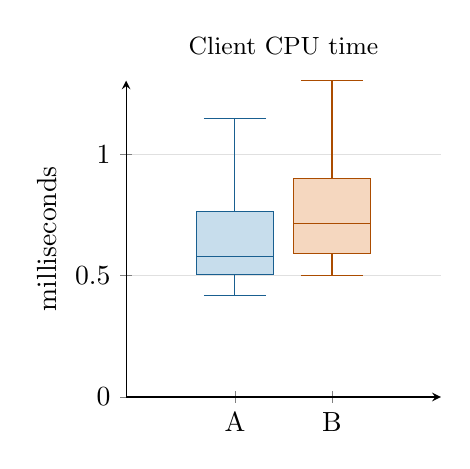
\begin{tikzpicture}
  \begin{axis}[boxplot/draw direction=y, width=0.46\linewidth, height=5.6cm,
      xtick={1,2}, xticklabels={A, B}, ymin=0, ylabel={milliseconds},
      title={\small Client CPU time}, axis lines=left, ymajorgrids, grid style={black!12},
      enlarge x limits=0.4]
    % Generated by prepare_data2.py. Do not edit.
\addplot+[boxplot prepared={draw position=1, lower whisker=0.4180, lower quartile=0.5045, median=0.5798, upper quartile=0.7646, upper whisker=1.1493}, fill=colorA!25, draw=colorA!80!black] coordinates {};
\addplot+[boxplot prepared={draw position=2, lower whisker=0.5008, lower quartile=0.5922, median=0.7157, upper quartile=0.9001, upper whisker=1.3045}, fill=colorB!25, draw=colorB!80!black] coordinates {};

  \end{axis}
\end{tikzpicture}\hfill
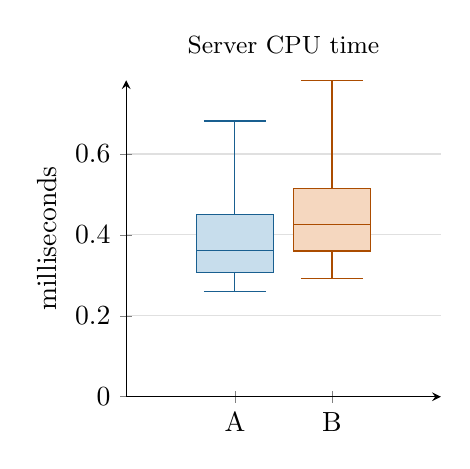
\begin{tikzpicture}
  \begin{axis}[boxplot/draw direction=y, width=0.46\linewidth, height=5.6cm,
      xtick={1,2}, xticklabels={A, B}, ymin=0, ylabel={milliseconds},
      title={\small Server CPU time}, axis lines=left, ymajorgrids, grid style={black!12},
      enlarge x limits=0.4]
    % Generated by prepare_data2.py. Do not edit.
\addplot+[boxplot prepared={draw position=1, lower whisker=0.2602, lower quartile=0.3078, median=0.3608, upper quartile=0.4503, upper whisker=0.6817}, fill=colorA!25, draw=colorA!80!black] coordinates {};
\addplot+[boxplot prepared={draw position=2, lower whisker=0.2921, lower quartile=0.3603, median=0.4248, upper quartile=0.5152, upper whisker=0.7822}, fill=colorB!25, draw=colorB!80!black] coordinates {};

  \end{axis}
\end{tikzpicture}
\caption{CPU time of one handshake. Box: 25th to 75th percentile with the median line; whiskers:
5th and 95th percentile. Blue = A, orange = B.}
\label{fig:cpubox}
\end{figure}

\FloatBarrier
\section{What crosses the wire}

Phase~1 has to show verified encryption and decryption, and a unit test on a socket pair is a weak
form of that. We therefore put a small TLS-aware proxy between the real client and server, and in
the same private namespace recorded the loopback interface to a real \prog{.pcap} file
(Figure~\ref{fig:wirerig}). The proxy reads the one part of TLS~1.3 that is not encrypted, the two
hello messages, and can flip a single bit in a chosen encrypted record. The packet capture gives
the headers; the proxy gives an independent count of the same bytes.

\begin{figure}[!tbp]
\centering
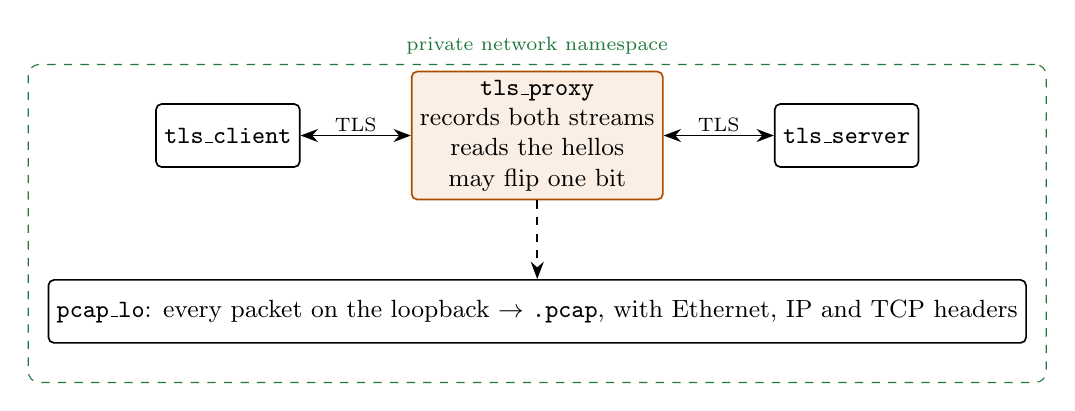
\begin{tikzpicture}[node distance=5mm and 14mm]
  \node[box] (cli) {\prog{tls\_client}};
  \node[box, fill=colorB!10, draw=colorB!80!black, right=of cli] (px) {\prog{tls\_proxy}\\records both streams\\reads the hellos\\may flip one bit};
  \node[box, right=of px] (srv) {\prog{tls\_server}};
  \draw[darr] (cli) -- node[lbl, above] {TLS} (px);
  \draw[darr] (px) -- node[lbl, above] {TLS} (srv);
  \node[box, below=10mm of px, minimum width=9.4cm] (cap) {\prog{pcap\_lo}: every packet on the loopback $\to$ \prog{.pcap}, with Ethernet, IP and TCP headers};
  \draw[arr, dashed] (px.south) -- (cap.north);
  \begin{scope}[on background layer]
    \node[draw=okgreen, dashed, rounded corners=4pt, fit=(cli)(srv)(cap), inner xsep=7pt, inner ysep=14pt,
          label={[font=\scriptsize, okgreen]above:private network namespace}] {};
  \end{scope}
\end{tikzpicture}
\caption{The test bench. The proxy sees the TLS stream; the capture sees the packets.}
\label{fig:wirerig}
\end{figure}

\subsection{What the capture shows}

In both configurations the first message from the client names exactly one key-exchange group, the
pinned one (\texttt{\WireAGroups} for A, \texttt{\WireBGroups} for B), offers TLS~1.3 only and one cipher
suite (\texttt{\WireASuite}). The server chooses the same group (\texttt{\WireAChosen},
\texttt{\WireBChosen}) with no retry, so nothing was negotiated down. After the two hello messages
every record is encrypted: the server's certificate cannot be read from the wire. None of the five
queued records, none of their sequence-number and time fields, and none of the server's ACKs appears
anywhere in the captured bytes, while the same records \emph{are} in the server's store, which shows
the search could have found them. The captured payload equals the proxy's own byte count in both
directions (A: \WireAAgree; B: \WireBAgree), so the two captures agree and no packet was counted twice.
Table~\ref{tab:wire} gives the byte totals with headers for a run of five records.

\begin{table}[!htbp]
\centering
\caption{One run, five records, on the wire. ``On the wire'' is the whole Ethernet frame. Headers add
\WireAOver{} bytes over \WireAPkts{} packets in A and \WireBOver{} over \WireBPkts{} in B;
the clean loopback had \WireARetx{} retransmissions in A and \WireBRetx{} in B.}
\label{tab:wire}
\small
\begin{tabular}{@{}llrrr@{}}
\toprule
Config & Direction & Packets & TLS payload, B & On the wire, B \\
\midrule
% Generated by prepare_data2.py. Do not edit.
A & client $\to$ server & 15 & 587 & 1573 \\
 & server $\to$ client & 7 & 950 & 1420 \\
B & client $\to$ server & 15 & 1763 & 2749 \\
 & server $\to$ client & 7 & 2038 & 2508
\\
\bottomrule
\end{tabular}
\end{table}

\subsection{Damaged records are refused (T09)}

Table~\ref{tab:tamper} shows the four places where the proxy flipped one bit. In every case TLS refused the
damaged record, nothing damaged was stored, and the record still arrived exactly once. Figure~\ref{fig:tamper}
shows the first case. A damaged ACK followed by the resend exercises two requirements together: the
client must not trust the ACK, and the server must recognise the duplicate (T05 and T09).

\begin{table}[!htbp]
\centering
\caption{Where one bit was flipped, configuration B, and what happened.}
\label{tab:tamper}
\small
\begin{tabularx}{\linewidth}{@{}lX@{}}
\toprule
Damaged record & Result \\
\midrule
Client's \msg{record} & Server rejects it (authentication tag), stores nothing, sends no ACK; client reconnects and delivers; stored once, never the damaged bytes \\
Server's \msg{ack} & Client refuses it and reconnects; resends; server recognises the duplicate, ACKs again; stored once \\
Server's first encrypted handshake record & Client's handshake fails and the client stops: it fails closed and does not retry \\
Client's Finished & Server refuses the connection; the client notices when no ACK comes, reconnects and delivers \\
\bottomrule
\end{tabularx}
\end{table}

\begin{figure}[!tbp]
\centering
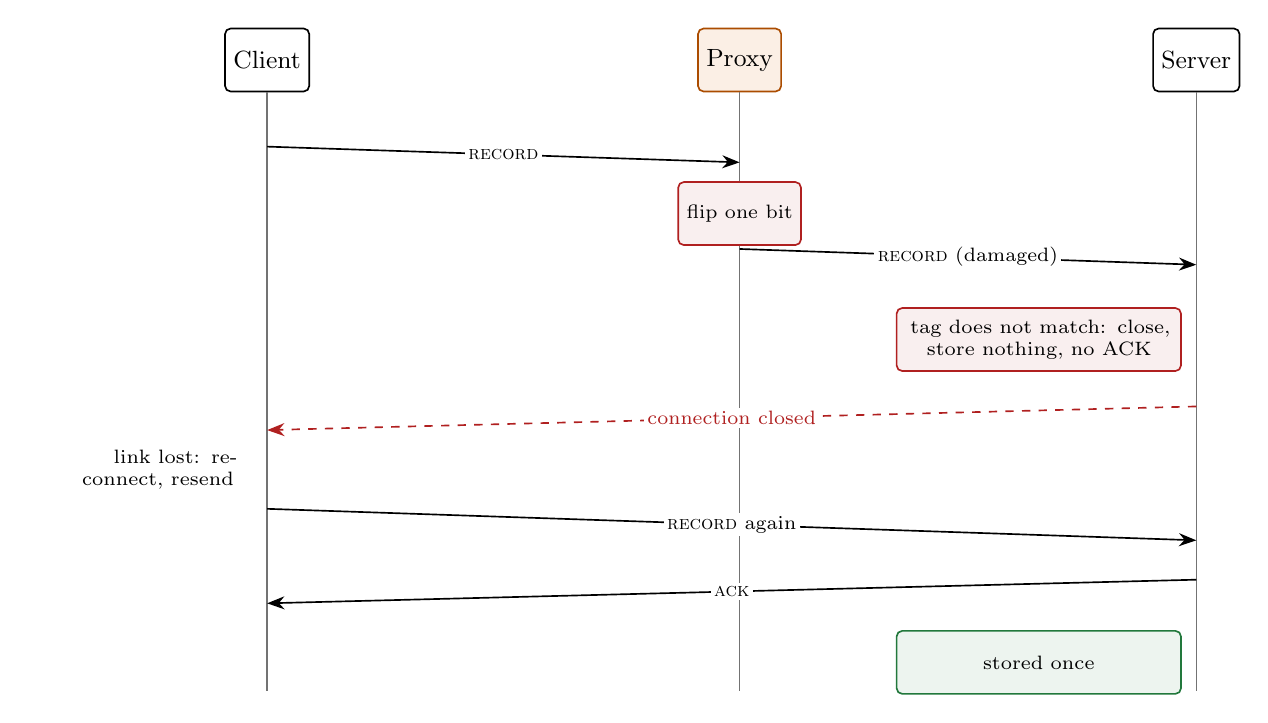
\begin{tikzpicture}[x=1cm,y=1cm]
  \node[box] (C) at (1.6,0) {Client};
  \node[box, fill=colorB!10, draw=colorB!80!black] (P) at (7.6,0) {Proxy};
  \node[box] (S) at (13.4,0) {Server};
  \foreach \n in {C,P,S} \draw[life] (\n.south) -- ++(0,-7.6);
  \draw[arr] (1.6,-1.1) -- node[lbl] {\msg{record}} (7.6,-1.3);
  \node[bad, font=\scriptsize] at (7.6,-1.95) {flip one bit};
  \draw[arr] (7.6,-2.4) -- node[lbl] {\msg{record} (damaged)} (13.4,-2.6);
  \node[bad, font=\scriptsize, text width=3.4cm] at (11.4,-3.55) {tag does not match: close, store nothing, no ACK};
  \draw[badarr] (13.4,-4.4) -- node[lbl] {connection closed} (1.6,-4.7);
  \node[font=\scriptsize, anchor=east, text width=2.5cm, align=right] at (1.3,-5.2) {link lost: reconnect, resend};
  \draw[arr] (1.6,-5.7) -- node[lbl] {\msg{record} again} (13.4,-6.1);
  \draw[arr] (13.4,-6.6) -- node[lbl] {\msg{ack}} (1.6,-6.9);
  \node[done, font=\scriptsize, text width=3.4cm] at (11.4,-7.65) {stored once};
\end{tikzpicture}
\caption{A damaged \msg{record}. The proxy damages the first connection only.}
\label{fig:tamper}
\end{figure}

\section{Preparing Phase 2 without hardware}

The Pico side is not built, but its software contract can be fixed and tested now. The UART frame between
Pico~A and Pi~A (Figure~\ref{fig:frame}) is 21 bytes for one sample. A single C file builds and parses it,
and \emph{both} the Pico firmware (with the Pico SDK) and Pi~A compile that same file
(Figure~\ref{fig:shared}), so the two ends cannot disagree about the format.

\begin{figure}[!tbp]
\centering
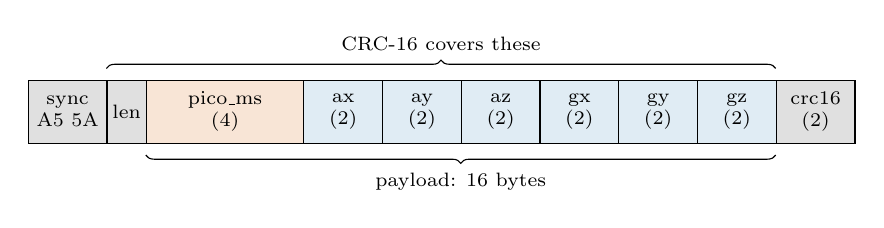
\begin{tikzpicture}[x=0.5cm,y=1cm]
  \tikzset{f/.style={draw, minimum height=8mm, font=\scriptsize, align=center, inner sep=0pt, anchor=west}}
  \node[f, minimum width=1.0cm, fill=black!12] at (0,0) {sync\\A5 5A};
  \node[f, minimum width=0.5cm, fill=black!12] at (2,0) {len};
  \node[f, minimum width=2.0cm, fill=colorB!16] at (3,0) {pico\_ms\\(4)};
  \foreach \i/\n in {0/ax,1/ay,2/az,3/gx,4/gy,5/gz}
    \node[f, minimum width=1.0cm, fill=colorA!14] at (7+2*\i,0) {\n\\(2)};
  \node[f, minimum width=1.0cm, fill=black!12] at (19,0) {crc16\\(2)};
  \draw[decorate, decoration={brace, amplitude=3pt, mirror}] (3,-0.55) -- node[below=3pt, font=\scriptsize] {payload: 16 bytes} (19,-0.55);
  \draw[decorate, decoration={brace, amplitude=3pt}] (2,0.55) -- node[above=3pt, font=\scriptsize] {CRC-16 covers these} (19,0.55);
\end{tikzpicture}
\caption{One sample on the UART, 21 bytes, big-endian. Widths are proportional to bytes.}
\label{fig:frame}
\end{figure}

\begin{figure}[!tbp]
\centering
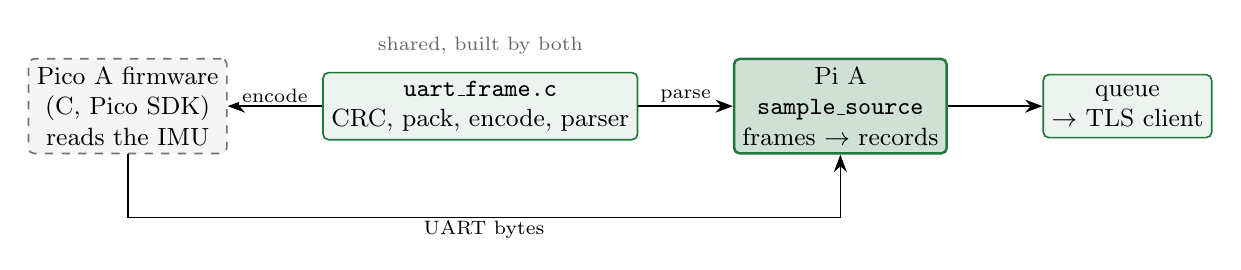
\begin{tikzpicture}[node distance=6mm and 12mm]
  \node[done, minimum width=3.4cm] (u) {\prog{uart\_frame.c}\\CRC, pack, encode, parser};
  \node[todo, left=of u] (pico) {Pico A firmware\\(C, Pico SDK)\\reads the IMU};
  \node[newd, right=of u] (pi) {Pi A\\\prog{sample\_source}\\frames $\to$ records};
  \node[done, right=of pi] (q) {queue\\$\to$ TLS client};
  \draw[arr] (u) -- node[lbl, above] {encode} (pico);
  \draw[arr] (u) -- node[lbl, above] {parse} (pi);
  \draw[arr] (pi) -- (q);
  \draw[arr] (pico.south) |- ++(0,-8mm) -| node[lbl, pos=0.25, below] {UART bytes} (pi.south);
  \node[font=\scriptsize, text=black!60, above=1mm of u] {shared, built by both};
\end{tikzpicture}
\caption{One file for both ends. The firmware part (dashed) is Phase~2.}
\label{fig:shared}
\end{figure}

\subsection{Surviving a damaged cable}

The parser keeps a window of at most 37 bytes (the longest frame). When a candidate frame fails its
check, it drops only the \emph{first} byte and looks again, so the bytes behind a damaged frame are
searched for the next real frame (Figure~\ref{fig:window}). A lost byte, an extra byte or a false sync
pattern therefore costs only the damaged frame. A parser that discards the whole claimed frame would also
lose the good frames it swallowed. Tests cover every possible single-bit flip of a frame, every possible lost
byte, inserted bytes at every position, random noise, and a 300{,}000-byte random stream.

\begin{figure}[!tbp]
\centering
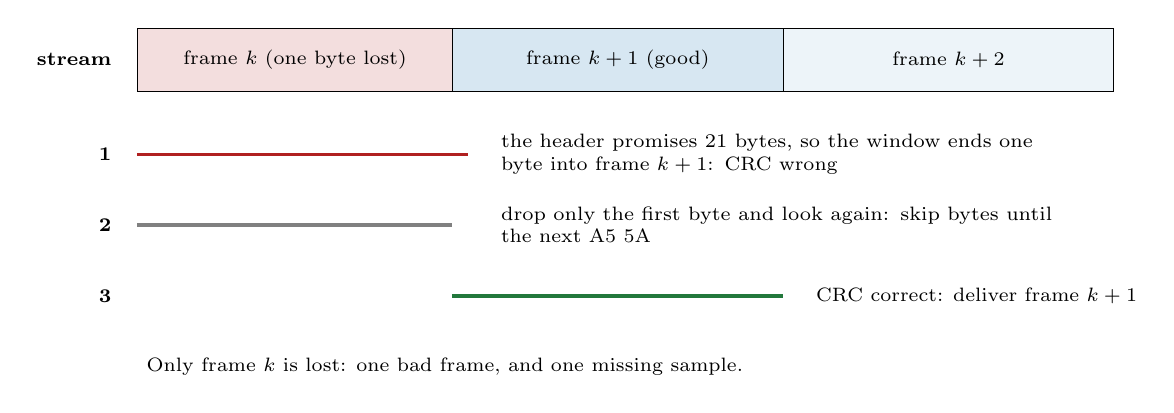
\begin{tikzpicture}[x=1cm,y=1cm]
  \tikzset{seg/.style={draw, minimum height=8mm, font=\scriptsize, inner sep=0pt, anchor=west, align=center}}
  \node[font=\scriptsize\bfseries, anchor=east] at (-0.2,0) {stream};
  \node[seg, minimum width=4.0cm, fill=badred!15] at (0,0) {frame $k$ (one byte lost)};
  \node[seg, minimum width=4.2cm, fill=colorA!18] at (4.0,0) {frame $k+1$ (good)};
  \node[seg, minimum width=4.2cm, fill=colorA!8] at (8.2,0) {frame $k+2$};
  \node[font=\scriptsize\bfseries, anchor=east] at (-0.2,-1.2) {1};
  \draw[line width=1.2pt, badred] (0,-1.2) -- (4.2,-1.2);
  \node[font=\scriptsize, anchor=west, text width=7.2cm] at (4.5,-1.2) {the header promises 21 bytes, so the window ends one byte into frame $k+1$: CRC wrong};
  \node[font=\scriptsize\bfseries, anchor=east] at (-0.2,-2.1) {2};
  \draw[line width=1.2pt, black!50] (0,-2.1) -- (4.0,-2.1);
  \node[font=\scriptsize, anchor=west, text width=7.2cm] at (4.5,-2.1) {drop only the first byte and look again: skip bytes until the next A5 5A};
  \node[font=\scriptsize\bfseries, anchor=east] at (-0.2,-3.0) {3};
  \draw[line width=1.2pt, okgreen] (4.0,-3.0) -- (8.2,-3.0);
  \node[font=\scriptsize, anchor=west] at (8.5,-3.0) {CRC correct: deliver frame $k+1$};
  \node[font=\scriptsize, anchor=west] at (0,-3.9) {Only frame $k$ is lost: one bad frame, and one missing sample.};
\end{tikzpicture}
\caption{Re-synchronisation after a lost byte.}
\label{fig:window}
\end{figure}

\subsection{Counting missing samples}

Pi~A turns each good frame into the start of a record (the queue adds the sequence number) and counts
what went wrong. Missing samples are found from the Pico's own timestamp \prog{pico\_ms}, with unsigned
32-bit subtraction so the wrap at $2^{32}$ is not a gap (Figure~\ref{fig:gaps}). A jump of ten seconds
or more, or time going backwards, is a restart of the Pico, not millions of lost samples. In a test of
1200 frames with some dropped and some damaged, the count of lost samples equalled the number dropped plus
the number damaged exactly. One caution: the record's timestamp \prog{ts\_ms} is when Pi~A \emph{read} the
frame, not when the Pico sampled, because the driver holds bytes until they are read.

\begin{figure}[!tbp]
\centering
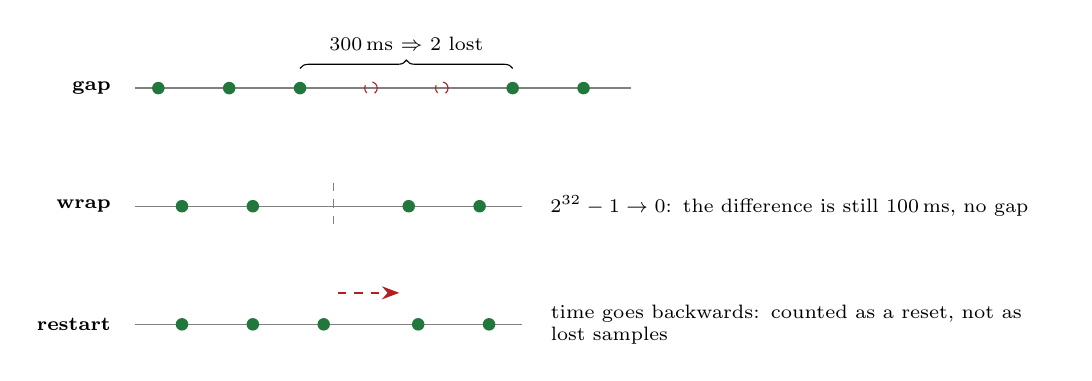
\begin{tikzpicture}[x=0.6cm,y=1cm]
  \tikzset{tick/.style={line width=0.6pt}, got/.style={circle, fill=okgreen, inner sep=1.6pt},
           lost/.style={circle, draw=badred, dashed, inner sep=1.6pt}}
  % on time with a gap
  \node[font=\scriptsize\bfseries, anchor=east] at (-0.3,0) {gap};
  \draw[line width=0.5pt, black!50] (0,0) -- (10.5,0);
  \foreach \x in {0,1,2} \node[got] at (\x*1.5+0.5,0) {};
  \node[lost] at (5,0) {}; \node[lost] at (6.5,0) {};
  \node[got] at (8,0) {}; \node[got] at (9.5,0) {};
  \draw[decorate, decoration={brace, amplitude=3pt}] (3.5,0.25) -- node[above=3pt, font=\scriptsize] {300\,ms $\Rightarrow$ 2 lost} (8,0.25);
  % wrap
  \node[font=\scriptsize\bfseries, anchor=east] at (-0.3,-1.5) {wrap};
  \draw[line width=0.5pt, black!50] (0,-1.5) -- (8.2,-1.5);
  \node[got] at (1,-1.5) {}; \node[got] at (2.5,-1.5) {};
  \draw[dashed, black!50] (4.2,-1.2) -- (4.2,-1.8);
  \node[got] at (5.8,-1.5) {}; \node[got] at (7.3,-1.5) {};
  \node[font=\scriptsize, anchor=west, text width=6.4cm] at (8.6,-1.5) {$2^{32}-1 \to 0$: the difference is still 100\,ms, no gap};
  % reset
  \node[font=\scriptsize\bfseries, anchor=east] at (-0.3,-3.0) {restart};
  \draw[line width=0.5pt, black!50] (0,-3.0) -- (8.2,-3.0);
  \node[got] at (1,-3.0) {}; \node[got] at (2.5,-3.0) {}; \node[got] at (4,-3.0) {};
  \draw[badarr] (4.3,-2.6) -- (5.6,-2.6);
  \node[got] at (6,-3.0) {}; \node[got] at (7.5,-3.0) {};
  \node[font=\scriptsize, anchor=west, text width=6.4cm] at (8.6,-3.0) {time goes backwards: counted as a reset, not as lost samples};
\end{tikzpicture}
\caption{Gap rules. Filled: received. Dashed: never arrived.}
\label{fig:gaps}
\end{figure}

\section{How the work is checked}

Every module has a plain C test program and the end-to-end scripts start the real client and server as
separate processes. Besides the happy path, each new feature has an adversarial test: wrong length, damaged
input, a partial write, an existing file that must not be overwritten, a process that must not hang.
Table~\ref{tab:tests} groups what the \NTests{} automated tests cover. We also break the code on purpose (a
\emph{mutation}: an off-by-one, a check removed, a wrong byte order) and confirm that a test fails; this
caught several tests that passed for the wrong reason. Code is built with all warnings as errors, with
address and undefined-behaviour sanitizers, and tests that use timing or pseudo-terminals are repeated 40
times to rule out flakes.

\begin{table}[!htbp]
\centering
\caption{Test areas.}
\label{tab:tests}
\small
\begin{tabularx}{\linewidth}{@{}lX@{}}
\toprule
Area & Covers \\
\midrule
Wire format, UART frame & Byte vectors, every bit flip, lost and extra bytes, noise, false sync \\
Store, queue & File layout, restart, torn last entry, damage, full, ACKs in any order, compaction, a model test \\
TLS link, client, server & A and B, downgrade, wrong hostname, untrusted CA, tampered record, timeout, replay, outage, restart \\
Loss and cost runners & Delivery verdicts, percentiles, server and client byte agreement, netem really acting \\
Wire and capture & Pinned group on the wire, no plaintext, damaged records refused, capture equals proxy count \\
Sample source & Raw serial mode (all 256 byte values), gap rules, 1200-frame accounting, port timeout and disconnect \\
\bottomrule
\end{tabularx}
\end{table}

\section{What remains to close Phase 1}

Figure~\ref{fig:road} shows the road. The software is essentially complete. What remains is running the
measurements at full size, writing them up, and the advisor's review, which is also the gate to Phase~2.

\begin{figure}[!tbp]
\centering
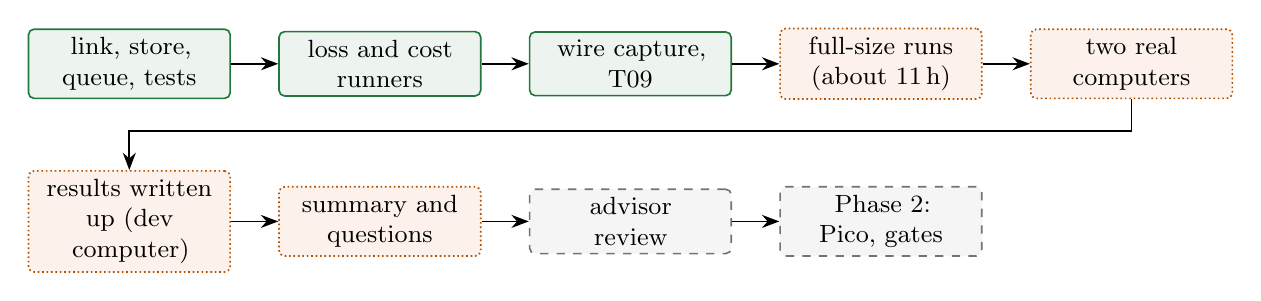
\begin{tikzpicture}[node distance=5mm and 6mm, every node/.append style={font=\scriptsize, text width=2.35cm, align=center}]
  \node[done] (a) {link, store,\\queue, tests};
  \node[done, right=of a] (b) {loss and cost\\runners};
  \node[done, right=of b] (c) {wire capture,\\T09};
  \node[next, right=of c] (d) {full-size runs\\(about 11\,h)};
  \node[next, right=of d] (e) {two real\\computers};
  \node[next, below=9mm of a] (f) {results written\\up (dev computer)};
  \node[next, right=of f] (g) {summary and\\questions};
  \node[todo, right=of g] (h) {advisor\\review};
  \node[todo, right=of h] (i) {Phase 2:\\Pico, gates};
  \foreach \x/\y in {a/b, b/c, c/d, d/e, f/g, g/h, h/i} \draw[arr] (\x) -- (\y);
  \draw[arr] (e.south) -- ++(0,-4mm) -| ($(f.north)+(0,0mm)$);
\end{tikzpicture}
\caption{Remaining steps. Solid: done. Dotted: next. Dashed: waits for the advisor.}
\label{fig:road}
\end{figure}

\subsection{Questions for the advisor}

\begin{itemize}\setlength\itemsep{0pt}
\item \textbf{Pico role.} We understand the Pico~2 or Pico~W does only sensor and display I/O and all TLS stays
      on the Pi~4B, because the Pico cannot run TLS. The advisor's wording of ``migration to Pico~W'' could be read
      as a platform change; please confirm.
\item Q5: which instrument for current and power, and is per-handshake energy needed? This decides whether a sensor is bought.
\item Q10: is packet loss emulated with \prog{tc netem} on the Pis or at the access point?
\item Q11: may the Pi services stay in C?
\item Q6 and Q8: confirm there is no rekey and no command channel.
\item Q15: should the existing logger be reused for the evidence files?
\item Confirm the queue size of 10{,}000 records and the reject-new rule.
\end{itemize}

\FloatBarrier
\section{Claims and limits}

Hybrid key establishment protects the \emph{key exchange} against a future quantum computer. It is
\textbf{not} post-quantum authentication: the baseline authenticates with an ordinary classical certificate,
and this report says so wherever it matters. This is an educational Wi-Fi link, not flight-approved, not
space-qualified and not endorsed by any agency. All measurements here come from one development computer
over loopback; they show that the harnesses work and give a first idea of the sizes and costs. They must not
be quoted as results for the Raspberry Pi~4B or the Pico, and they are not gate evidence.

\appendix
\section{Reproducing the numbers}

Every number in Sections~4 to~6 is generated from raw files by \prog{prepare\_data2.py}; nothing is typed.

\begin{small}
\begin{verbatim}
cmake -S . -B build -DCMAKE_BUILD_TYPE=Release -DOPENSSL_ROOT_DIR=$HOME/opt/openssl-3.5.9
cmake --build build && ctest --test-dir build
scripts/run_handshake_bench.sh $HOME/opt/openssl-3.5.9 build \
    experiments/configs/t10_handshake_loopback.conf results/
scripts/run_loss_test.sh $HOME/opt/openssl-3.5.9 build \
    experiments/configs/t08_loss_loopback.conf results/
scripts/capture_demo.sh $HOME/opt/openssl-3.5.9 build results/wire_demo
python3 -I docs/report/prepare_data2.py results results/wire_demo \
    docs/report/data2 build
cd docs/report && latexmk -pdf progress_report_2.tex
\end{verbatim}
\end{small}

\end{document}
